
如何划分和识别区域是当前研究中的一个难点,也是计算区域转移矩阵的基础。现有研究中的区域识别有简单的讲区域划分为$n\times m$的网格,这种情况下当网格的粒度变大,其计算复杂度也急剧上升。对于$n\times m$的网格来说,其计算区域转移矩阵的复杂度为$O(n^2 \times m^2)$。另一种常用方式是通过手动的划分,对区域的按照某个属性(例如小区)划分。这种划分方式对于特定情境较为符合,但是可扩展性不强,且带有较大的主观性。
因此为了保证区域转移概率的准确度,计算效率以及可扩展性,我们采用了讲区域划分为细粒度的网格后再进行聚类。

此外我们区域按照不同时段以及不同的事件类型动态划分。
首先,我们
\begin{definition}
\label{cell}
\textbf{格子为区域识别中的最小单位,规定某块区域的范围,也表示一段连续经纬度的集合。}本文将之定义为矩形格子。记为:
\begin{equation}
C_{x,y}::=\{(lon,lat)|x \le \frac{{lon}}{{X}} < x + 1,
y \le \frac{{lat}}{{Y}} < y + 1\}.
\end{equation}
\end{definition}


其中,$C_{x,y}$ 表示编号为$(x,y)$的格子,$lon$ 和 $lat$ 表示经度和纬度,$X$和$Y$表示经度和纬度方向上每个格子的长度。基于格子可以定义区域。

\begin{definition}
\label{def_region}
\textbf{区域是一些连续格子的集合,在本文中,也是区域转移概率矩阵计算的最小单位。}记为:

\begin{equation}
R_m:: = \{ C_{i,j}|if C_{x,y} \in R_m
\Rightarrow \|x - i\| \le 1,\|y - j\| \le 1\}.
\end{equation}

\end{definition}

我们按照对应时间段对应事件发生的事件数对之进行划分。由于事件分布及其不均匀,我们同时也规定了两种区域,一种是事件密集区域,一种是事件稀疏区域。当区域中的每个格子的事件数均大于阈值$\eta$时,该区域为密集区域,否则为稀疏区域。事件密集区域为$\_top$个,为了减少密集区域仅包含一个或少数几个格子。同时为了保证区域大小不至于过大,我们定义了一个区域最多包含$ClusterSize$个格子,即$\|R_i\|\leq ClusterSize$。

对于某个时段的某一事件类别,我们首先计算每个格子发生的该类别事件数。首先需要找出$\_top$个密集区域,我们先降序排序,从事件最密集的格子开始,进行广度遍历,如果事件数大于$\eta$,则加入区域中,每个格子属于且仅属于一个区域。找到$\_top$个区域后,我们剩下的格子内的事件数不需要大于$_eta$,仅需要满足$\|R_i\|\leq ClusterSize$.

$\eta$设为整个场景中应时间段和事件类型的事件数的均值的两倍,区域识别的相关参数如下表\ref{table_region_rec},区域识别的具体算法见附录.


\begin{table}
\caption{区域识别相关参数}\label{table_region_rec}
\centering
\begin{tabular}{l|c|c|c|c}
  \hline
  Item & 0:00-8:59 &9:00-12:59&13:00-20:59 &21:00-23:59 \\
  \hline
  $\eta_{drop}$ & 56&84 &180 &51\\
  $\eta_{load}$ & 58&84 &182 &51\\
  \_top & 200&200 &200 &200\\
  clusterSize& 500&500 &500 &500\\
  \hline
\end{tabular}
\end{table}


\begin{figure}[ht]
\centering
\subfigure[drop event regions]{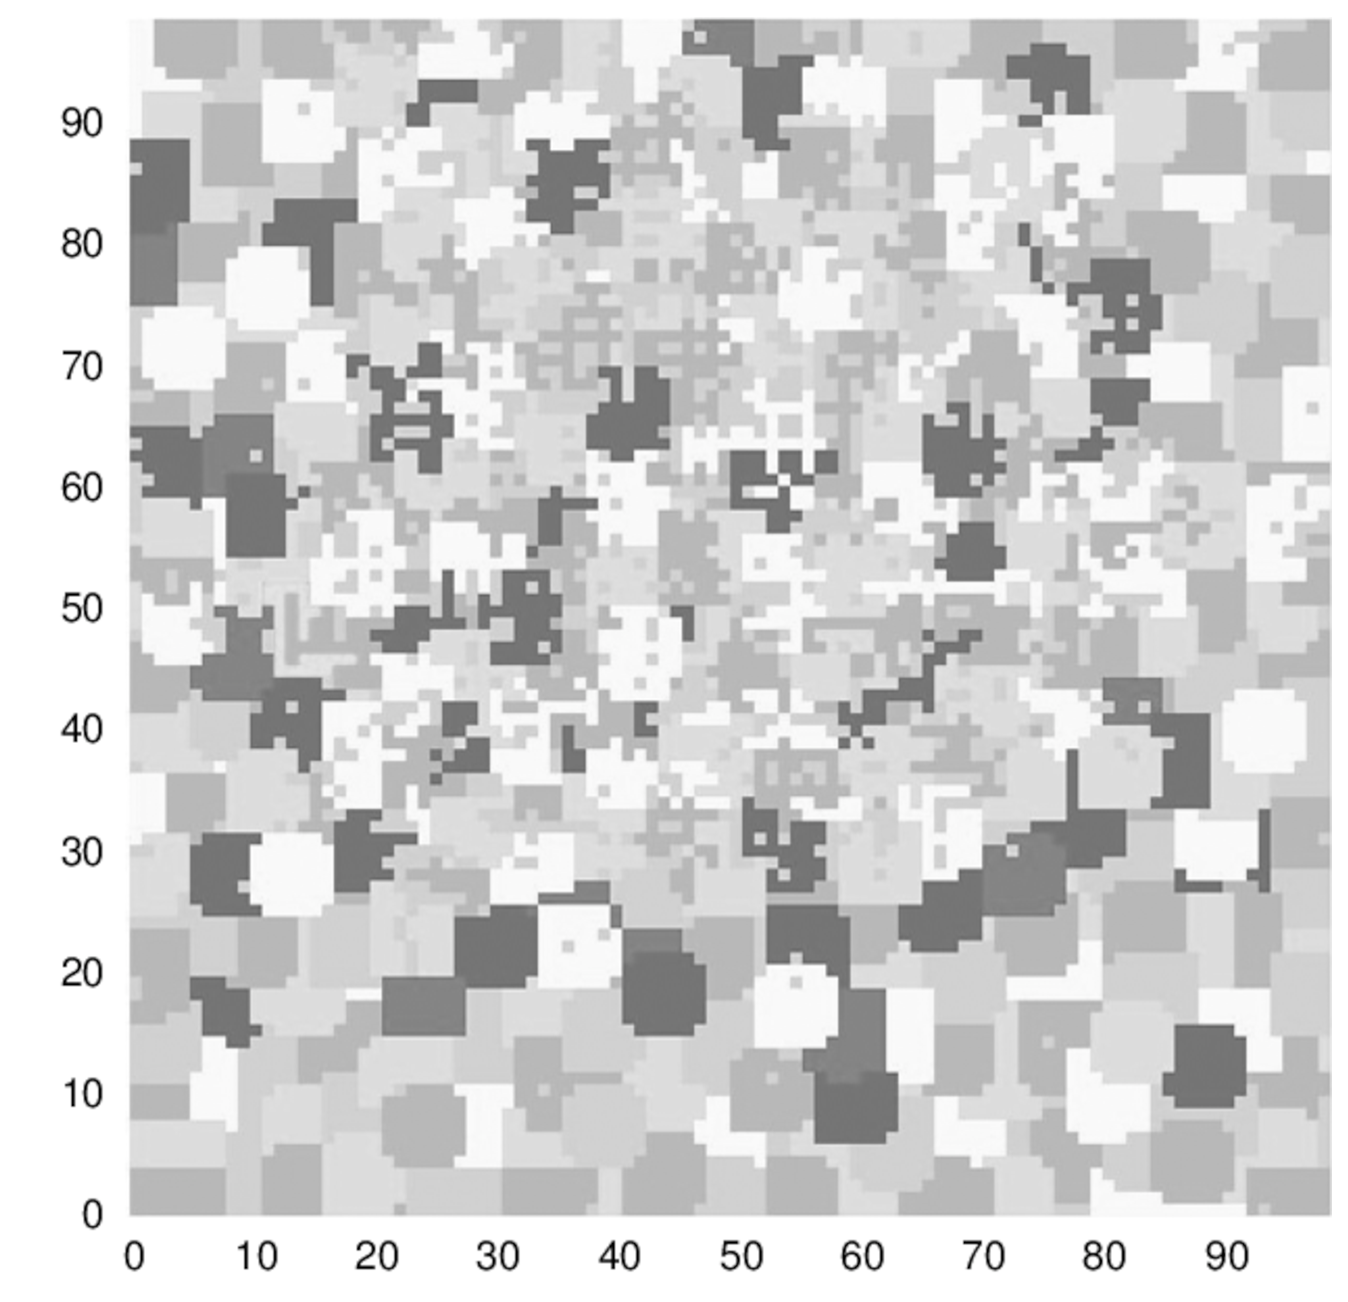
\includegraphics[width=0.23\textwidth]{figures/region/Areas-2011_event01.eps}}
\subfigure[load event regions]{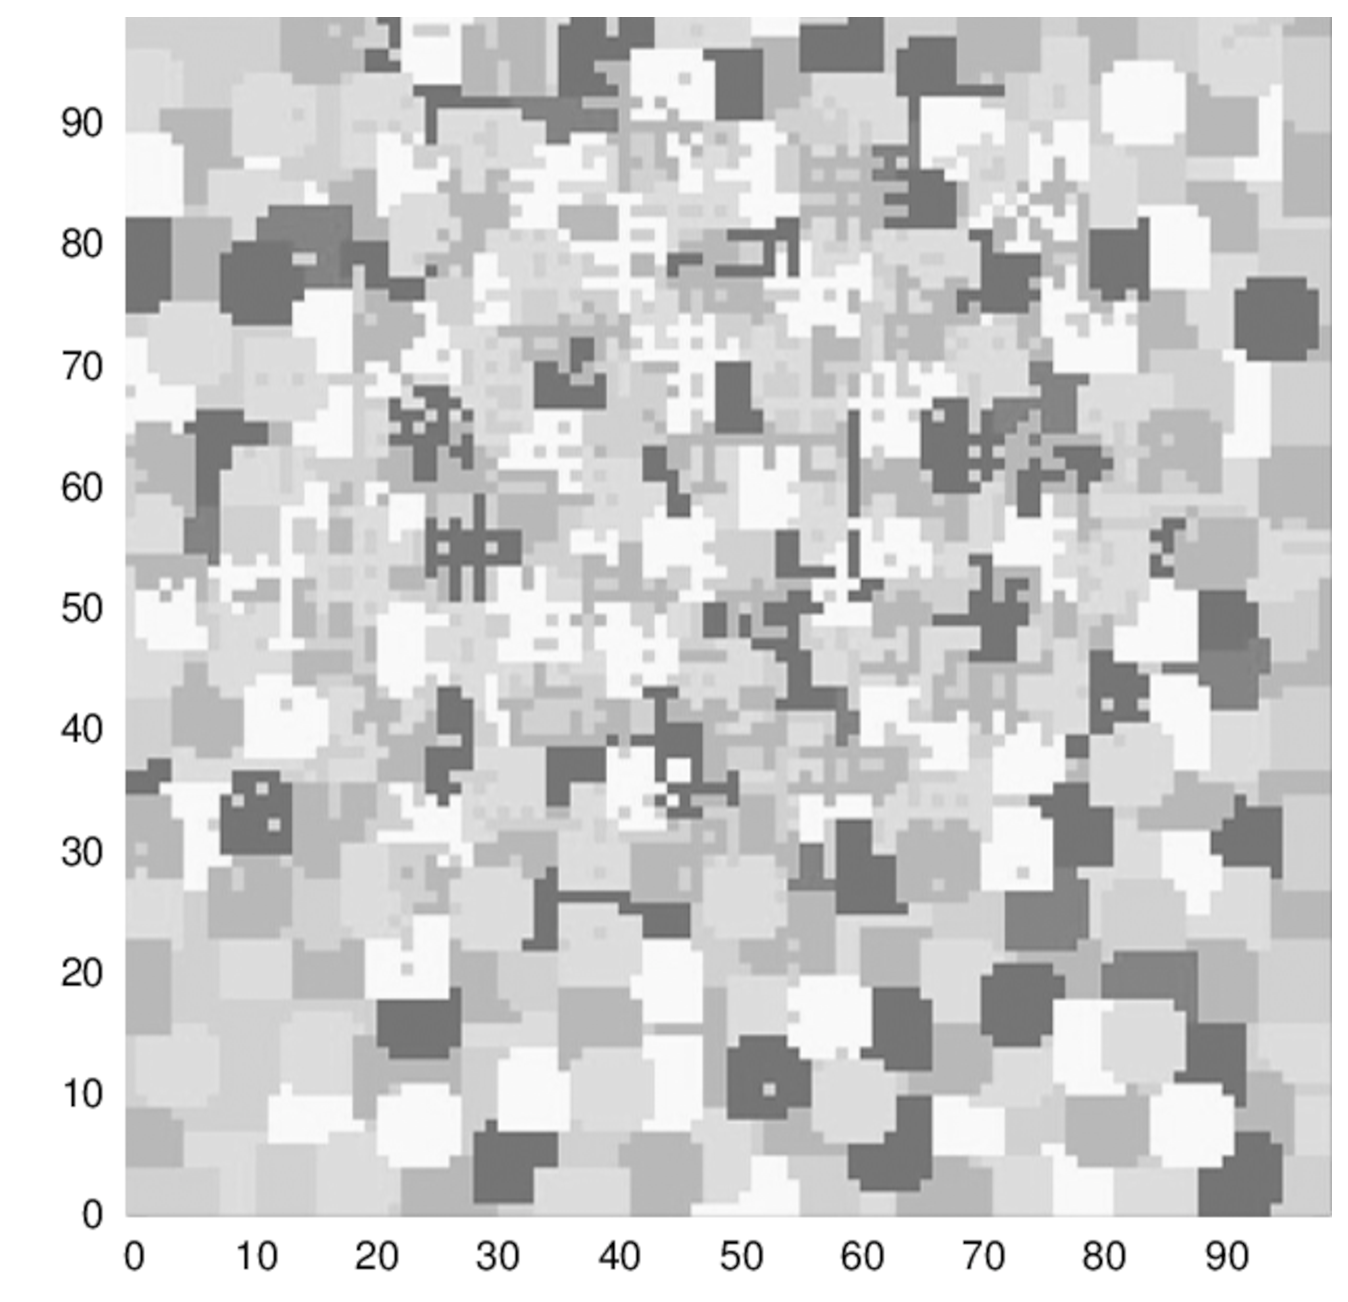
\includegraphics[width=0.23\textwidth]{figures/region/Areas-2011_event03.eps}}
\centering
\caption{Region recognition}\label{figure_region_recognizition}
\end{figure}

区域识别的结果如图\ref{figure_region_recognizition},其中每个色块都代表一个区域,由图可知,北京市的事件分布主要集中在主干道路上,其他较为规则的区域为稀疏区域,主要分布在城市周边。


